\documentclass[tikz,border=6pt]{standalone}
\usepackage{tikz}
\begin{document}
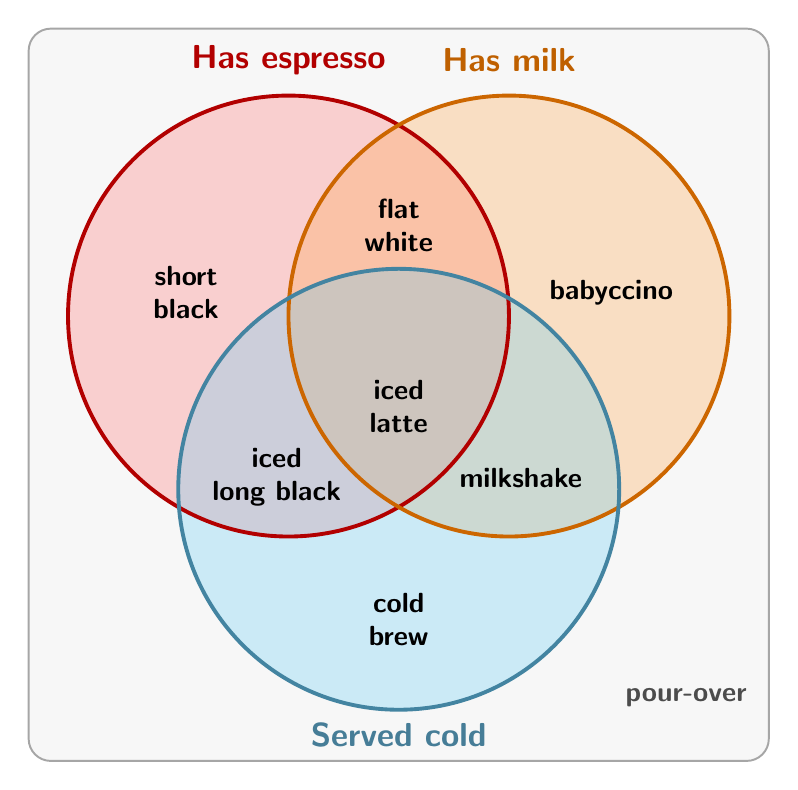
\begin{tikzpicture}[font=\sffamily]

  % Universe (so the ``none of the three'' region is visible)
  \draw[draw=black!35, fill=black!3, rounded corners=8pt, line width=0.7pt]
    (-4.7,-4.75) rectangle (4.7,4.55);


  % Circle geometry
  \def\r{2.8}
  \coordinate (E) at (-1.4,0.9);   % Has espresso
  \coordinate (M) at ( 1.4,0.9);   % Has milk
  \coordinate (C) at ( 0,-1.3);    % Served cold

  % Filled circles (transparency makes the overlaps show)
  \fill[red!55,    opacity=0.30] (E) circle (\r);
  \fill[orange!70, opacity=0.30] (M) circle (\r);
  \fill[cyan!60,   opacity=0.30] (C) circle (\r);

  % Outlines
  \draw[line width=1.4pt, draw=red!70!black]    (E) circle (\r);
  \draw[line width=1.4pt, draw=orange!80!black] (M) circle (\r);
  \draw[line width=1.4pt, draw=cyan!60!black]   (C) circle (\r);

  % Circle labels, placed on the non-overlapping arcs
  \node[font=\sffamily\bfseries\large, text=red!70!black]
    at (-1.4,4.15) {Has espresso};
  \node[font=\sffamily\bfseries\large, text=orange!75!black]
    at (1.4,4.15) {Has milk};
  \node[font=\sffamily\bfseries\large, text=cyan!55!black]
    at (0,-4.42) {Served cold};

  % --- Drinks, one per region ---

  % Espresso only
  \node[align=center, font=\sffamily\bfseries] at (-2.7,1.2) {short\\black};

  % Milk only
  \node[align=center, font=\sffamily\bfseries] at (2.7,1.2) {babyccino};

  % Cold only
  \node[align=center, font=\sffamily\bfseries] at (0,-2.95) {cold\\brew};

  % Espresso + milk, not cold
  \node[align=center, font=\sffamily\bfseries] at (0,2.05) {flat\\white};

  % Espresso + cold, no milk
  \node[align=center, font=\sffamily\bfseries] at (-1.55,-1.15) {iced\\long black};

  % Milk + cold, no espresso
  \node[align=center, font=\sffamily\bfseries] at (1.55,-1.15) {milkshake};

  % All three
  \node[align=center, font=\sffamily\bfseries] at (0,-0.25) {iced\\latte};

  % None of the three (outside all circles)
  \node[align=center, font=\sffamily\bfseries, text=black!70]
    at (3.65,-3.95) {pour-over};

\end{tikzpicture}
\end{document}
